\begin{frame}[hasprev=false, hasnext=true, fragile]
\label{example:program-graph}
\frametitle{Program graph}

\begin{lstlisting}
q = 1;
b = 2;
c = 3;
if (a ==2) {
   x = x + 2;
}  else {
   x = x / 2;
}
p = q / r;
if (b/c>3) {
   z = x + y;
}
\end{lstlisting}
\end{frame}


\begin{frame}[hasprev=true, hasnext=false, fragile, c]
\frametitle{Program graph}

\begin{figure}
	\centering
	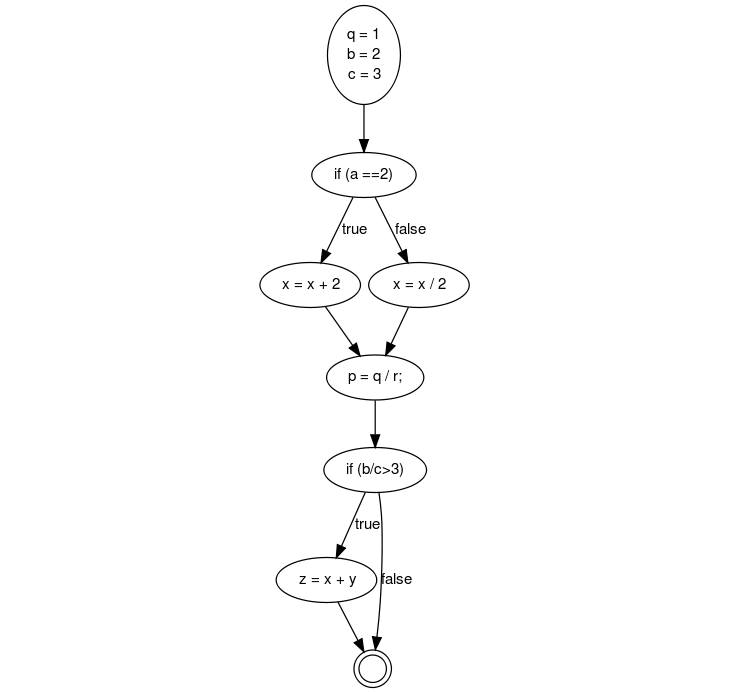
\includegraphics[scale=.3]{aux/examples/program-graph/cfg-example1}
\end{figure}
\end{frame}
